\documentclass{beamer}

\newcommand\hmmax{0}
\newcommand\bmmax{0}

\usepackage[utf8]{inputenc}
\usepackage[T1]{fontenc}
\usepackage{ae} % for pdf files
\usepackage[english]{babel}
\usepackage{lmodern}
\usepackage{geometry}
\usepackage{mathrsfs}
\usepackage{upgreek}
\usepackage{multicol}
\usepackage{verbatim}
\usepackage{amsmath,amsthm,amssymb}
\usepackage{bm}
%\usepackage{enumitem}
\usepackage{cancel} % for strikeout
\usepackage{xspace} % for spaces after commands
\usepackage{extpfeil} % for arrows
\usepackage{tikz}
\usepackage{beamerthemesplit}

\newtheorem{remark}{Remark}
\newtheorem{proposition}{Proposition}

% Commands
% Sets commands

% empty set
\newcommand{\eset}{\varnothing}

% set difference
\newcommand{\sub}{\setminus}

% set of elements
\newcommand{\set}[1]{\left\{#1\right\}}

% small set
\newcommand{\setsm}[1]{\{#1\}}

% builder separator
\newcommand{\bdsep}{\mathrel{}\middle|\mathrel{}}

% set builder notation
\newcommand{\setbd}[2]{\left\{#1\bdsep#2\right\}}

% set names
\newcommand{\setA}{A}
\newcommand{\setB}{B}
\newcommand{\setC}{C}
\newcommand{\setS}{S}

% elements names
\newcommand{\ea}{a}
\newcommand{\eb}{b}
\newcommand{\ec}{c}
\newcommand{\eo}{o}
\newcommand{\eap}{{a'}}
\newcommand{\ebp}{{b'}}
\newcommand{\ecp}{{c'}}

\newcommand{\eaa}[1]{\ea_{#1}}
\newcommand{\ebb}[1]{\eb_{#1}}
\newcommand{\ecc}[1]{\ec_{#1}}


% cardinality
\newcommand{\card}[1]{\left|#1\right|}

% powerset
\newcommand{\pset}[1]{\wp{#1}}

% set of nonempty subsets
\newcommand{\nepset}[1]{\wp^{+}{#1}}

% set of subsets of given cardinality
\newcommand{\cpset}[2]{\wp^{#1}{#2}}

% cardinal numbers names
\newcommand{\cardk}{\kappa}

% cartesian product
\newcommand{\cprod}{\times}

% Mathematical sets
\newcommand{\MathSet}[1]{\mathbb{#1}}
% Relations commands

% Relation names
\newcommand{\relR}{R}
\newcommand{\relS}{S}

% successors
\newcommand{\rsuc}[2]{#1[#2]}

% composition
\newcommand{\comp}{\circ}

% inverse
\newcommand{\inv}[1]{#1^{-1}}

% domain
\DeclareMathOperator{\dom}{dom}

% range
\DeclareMathOperator{\ran}{ran}
% Functions commands

% function names
\newcommand{\ff}{f}

% injective function
\newcommand{\ito}{\hookrightarrow}

% surjective function
\newcommand{\sto}{\twoheadrightarrow}

% bijective function
\newcommand{\bto}{\leftrightarrow}

% partial function
\newcommand{\pto}{\leadsto}

% identity
\DeclareMathOperator{\idOP}{id}
\newcommand{\id}[1]{\idOP_{#1}}

% characteristic function
\DeclareMathOperator{\chfunOP}{ch}
\newcommand{\chfun}[2]{\chfunOP_#2^#1}
% Sequences commands

% empty sequence
\newcommand{\eseq}{\varepsilon}

% sequence of elements
\newcommand{\seq}[1]{\left\langle #1 \right\rangle}

% small sequence
\newcommand{\seqsm}[1]{\langle #1 \rangle}

% sequence builder notation
\newcommand{\seqbd}[2]{\left\langle #1 \bdsep #2 \right\rangle}

% length
\newcommand{\len}[1]{\|#1\|}

% sequence names
\newcommand{\seqname}[1]{\mathrm{#1}}
\newcommand{\seqA}{\seqname{A}}
\newcommand{\seqB}{\seqname{B}}

% concatenation
\newcommand{\conc}{+}

\newcommand{\without}{-}

% indexes
\newcommand{\ii}{i}
\newcommand{\jj}{j}
\newcommand{\kk}{k}
\newcommand{\kkp}{{k'}}
% Numbers commands

% natural numbers
\newcommand{\Nats}{\MathSet{N}}

% positive natural numbers
\newcommand{\pNats}{\Nats^{+}}

% number names
\newcommand{\nn}{n}
\newcommand{\nm}{m}
\newcommand{\nv}{v}
\newcommand{\nonv}{{}}
\newcommand{\nr}{r}
\newcommand{\nrp}{{r'}}
% Tetration commands

\newcommand{\tetr}[3]{\exp_{#2}^{#1}(#3)}

\newcommand{\nx}{x}
\newcommand{\na}{a}
% Vectors commands

% n-vectors
\newcommand{\nVects}[1]{\Nats^{#1}}

\newcommand{\vectorname}[1]{\mathrm{#1}}

\newcommand{\vectv}{\vectorname{v}}
\newcommand{\vectvv}[1]{\vectv_{#1}}

\newcommand{\vectw}{\vectorname{w}}
\newcommand{\vectww}[1]{\vectw_{#1}}

% lexicographically smaller
\newcommand{\lexlt}{\prec}
% Permutations commands
\newcommand{\Perms}[1]{\MathSet{S}_{#1}}

% Permutation names
\newcommand{\permname}[1]{#1}

\newcommand{\permnu}{\permname{\nu}}
\newcommand{\permmu}{\permname{\mu}}
\newcommand{\perma}{\permname{\alpha}}
\newcommand{\permb}{\permname{\beta}}
% Bounds commands

% polynomials
\newcommand{\polyname}[1]{#1}
\newcommand{\polyp}{\polyname{p}}
% Alphabets commands

% alphabet names
\newcommand{\alphO}{\Omega}

% empty word
\newcommand{\eword}{\eseq}

% word names
\newcommand{\wordw}{w}

% Words over an alphabet
\newcommand{\Words}[1]{#1^{*}}

\newcommand{\neWords}[1]{#1^+}

\newcommand{\nWords}[2]{#1^{#2}}

% position
\newcommand{\posp}{p}
\newcommand{\posq}{q}
% Bits commands

\newcommand{\Bits}{\MathSet{B}}

\newcommand{\Bitstrings}{\neWords\Bits}

\newcommand{\tBitstrings}[1]{\Bits^{#1}}

\newcommand{\tBitnums}[1]{\Bits_{#1}}
\newcommand{\ntBitnums}[2]{\Bits_{#2}^{#1}}

% sizes of bitstrings
\newcommand{\tbit}{t}
\newcommand{\ubit}{u}

\newcommand{\Bitstringst}{\tBitstrings{\tbit}}
\newcommand{\Bitnumst}{\tBitnums{\tbit}}


% bitstring names
\newcommand{\bstrname}[1]{\mathrm{#1}}
\newcommand{\bstra}{\bstrname{a}}
\newcommand{\bstrb}{\bstrname{b}}

% bitsize
\newcommand{\bsz}[1]{\len{#1}}

% encoding
\newcommand{\benc}[1]{\overline{#1}}

% decoding
\newcommand{\bdec}[1]{\underline{#1}}

% largest t-bit number
\newcommand{\largtbit}[1]{N_{#1}}

% Symbol alphabet commands

% counting letter
\newcommand{\CL}{\mathcal{C}}

% logic letter
\newcommand{\LL}{\mathcal{L}}

% logical implication
\newcommand{\limp}{\rightarrow}

% logical equivalence
\newcommand{\lequ}{\leftrightarrow}

% any logcial connective
\newcommand{\anyconn}{\oplus}

% all logical connectives in order
\newcommand{\allconns}{\land,\lor,\limp,\lequ}

% any quantifier
\newcommand{\anyQ}{\mathsf{Q}}

% all quantifiers
\newcommand{\allQs}{\exists, \forall}

% symbol alphabet
\newcommand{\SymbAlph}{\alphO_{\CL}}

% counting quantifiers
\newcommand{\existsleq}[1]{\exists^{\leq#1}}
\newcommand{\existseq}[1]{\exists^{=#1}}
\newcommand{\existsgeq}[1]{\exists^{\geq#1}}

\newcommand{\miff}[2]{#1 \text{ iff } #2}
\newcommand{\mifff}[3]{#1 \text{ iff } #2 \text{ iff } #3}
% Variable symbols commands

\newcommand{\VarSymbs}{\mathcal{V}}

\newcommand{\varname}[1]{\bm{#1}}

\newcommand{\vv}[1]{\varname{v}_{#1}}
\newcommand{\xx}{\varname{x}}
\newcommand{\yy}{\varname{y}}
\newcommand{\zz}{\varname{z}}
\newcommand{\ww}{\varname{w}}

% generic variable symbols
\newcommand{\gvarname}[1]{#1}
\newcommand{\gx}{\gvarname{x}}
\newcommand{\gy}{\gvarname{y}}
\newcommand{\gxx}[1]{\gx_{#1}}
\newcommand{\gyy}[1]{\gy_{#1}}
% Signatures commands

% signatures
\newcommand{\signame}[1]{\mathrm{#1}}
\newcommand{\SigS}{\signame{\Sigma}}
\newcommand{\SigSp}{\signame{\Sigma'}}
\newcommand{\SigG}{\signame{\Gamma}}
\newcommand{\SigGp}{\signame{\Gamma'}}

% predicate symbols
\newcommand{\predname}[1]{\bm{#1}}
\newcommand{\pp}[1]{\predname{p}_{#1}}

% unary predicate symbols
\newcommand{\su}{\predname{u}}
\newcommand{\suu}[1]{\predname{u}_{#1}}

% equivalence predicate symbols
\newcommand{\se}{\predname{e}}
\newcommand{\see}[1]{\predname{e}_{#1}}

\newcommand{\sd}{\predname{d}}
\newcommand{\sdd}[1]{\predname{d}_{#1}}

\newcommand{\sle}{\predname{l}}
\newcommand{\slee}[1]{\predname{l}_{#1}}

% generic predicate symbol
\newcommand{\gpredname}[1]{#1}
\newcommand{\gp}{\gpredname{p}}
\newcommand{\gpp}[1]{\gp_{#1}}

% arity
\DeclareMathOperator{\ar}{ar}

% size of a signature
\newcommand{\sizename}[1]{#1}
\newcommand{\sizes}{\sizename{s}}
% Formulas commands

\newcommand{\FormulaSet}[2]{#1[#2]}

\newcommand{\Atomic}{\mathcal{A}t}

% Atomic formulas over a signature
\newcommand{\AtF}[1]{\FormulaSet{\Atomic}{#1}}

% Atomic formula grammar variable
\newcommand{\atfgv}{\alpha}

\newcommand{\Literal}{\mathcal{L}it}

% Literals over a signature
\newcommand{\LitF}[1]{\FormulaSet{\Literal}{#1}}

% Literal grammar variable
\newcommand{\litfgv}{\lambda}

% First-order formulas with counting
\newcommand{\Foc}{\mathcal{C}}

\newcommand{\FocF}[1]{\FormulaSet{\Foc}{#1}}

\newcommand{\focgv}{\varphi}

% First-order formulas
\newcommand{\Fo}{\mathcal{L}}

\newcommand{\FoF}[1]{\FormulaSet{\Fo}{#1}}

% any gorund logic
\newcommand{\aL}{\Lambda}

\newcommand{\aLF}[1]{\FormulaSet{\aL}{#1}}

% Formula names
\newcommand{\fphi}{\varphi}
\newcommand{\fphip}{{\fphi'}}
\newcommand{\fpsi}{\psi}
\newcommand{\fthe}{\theta}


% Variables occuring in a formula
\DeclareMathOperator{\vr}{vr}

\DeclareMathOperator{\fvr}{fvr}

% v-variable formulas
\newcommand{\vFoF}[2]{\FormulaSet{\Fo^{#1}}{#2}}

\newcommand{\vFocF}[2]{\FormulaSet{\Foc^{#1}}{#2}}

% r-rank first-order formulas
\newcommand{\rFoF}[2]{\FormulaSet{\Fo_{#1}}{#2}}

\newcommand{\rFocF}[2]{\FormulaSet{\Foc_{#1}}{#2}}

% r-rank v-variable formulas
\newcommand{\rvFoF}[3]{\FormulaSet{\Fo_{#1}^{#2}}{#3}}

\newcommand{\rvFocF}[3]{\FormulaSet{\Foc_{#1}^{#2}}{#3}}

% Quantifier rank glossary

% quantifier rank
\DeclareMathOperator{\qr}{qr}

% Structures commands

% structure names
\newcommand{\structurename}[1]{\mathfrak{#1}}

\newcommand{\StrA}{\structurename{A}}
\newcommand{\StrB}{\structurename{B}}
\newcommand{\StrAp}{\structurename{A'}}
\newcommand{\StrBp}{\structurename{B'}}
\newcommand{\StrBpp}{\structurename{B''}}
\newcommand{\StrAA}[1]{\StrA_{#1}}
\newcommand{\StrX}{\structurename{X}}
\newcommand{\StrXss}[1]{\StrX^{#1}}
\newcommand{\StrXs}{\StrXss\csps}
\newcommand{\StrXsij}[3]{\StrX^{#1}_{#2#3}}

% domain names
\newcommand{\domA}{A}
%\newcommand{\domAp}{{\domA'}}
\newcommand{\domAp}{A'}
\newcommand{\domB}{B}

\newcommand{\domXX}[1]{{#1\cprod #1}}

\newcommand{\domAA}{\domXX{A}}
\newcommand{\domBB}{\domXX{B}}

% iterpretation
\newcommand{\at}[2]{#2^{#1}}
% Standard translation commands

% standard translation
\DeclareMathOperator{\sttr}{st}
% Monadic two-variable satisfiability commands

\newcommand{\uUS}[1]{\US(#1)}
\newcommand{\eES}[1]{\ES(#1)}
\newcommand{\uesigS}[2]{\SigS(#1,#2)}
% Logic equivalence commands

% elementary equivalent structures
\newcommand{\elequiv}{\equiv}

% r-rank equivalent
\newcommand{\requiv}[1]{\equiv_{#1}}

% v-variable equivalent
\newcommand{\vequiv}[1]{\equiv^{#1}}

% r-rank v-variable equivalent
\newcommand{\rvequiv}[2]{\equiv_{#1}^{#2}}

% Logic games commands

% partial isomorphism
\newcommand{\pisoname}[1]{\mathfrak{#1}}

\newcommand{\pisop}{\pisoname{p}}
\newcommand{\pisoq}{\pisoname{q}}

% r-round EF game
\newcommand{\refG}[3]{G_{#1}(#2,#3)}

% r-round v-pebble game
\newcommand{\rvpbG}[4]{G_{#1}^{#2}(#3, #4)}

% a sequence of elements
\newcommand{\many}[1]{\bar{#1}}

% a set of partial isomorphisms
\newcommand{\pisoI}{\mathfrak{I}}
\newcommand{\pisoII}[1]{\mathfrak{I}_{#1}}

% support of a vector
\DeclareMathOperator{\supp}{supp}

% substitution
\newcommand{\vectsub}[3]{#1_{#2}^{#3}}

% Types commands

% The 1-types over S
\newcommand{\TpI}[1]{\Pi[#1]}

% 1-type name
\newcommand{\tpIp}{\pi}
\newcommand{\tpIpp}{{\pi'}}
\newcommand{\tpIr}{\rho}
\newcommand{\tpIrp}{{\rho'}}
\newcommand{\tpIk}{\kappa}
\newcommand{\tpIkp}{{\tpIk'}}
% dukes
\newcommand{\tpId}{\delta}
\newcommand{\tpIdp}{{\tpId'}}

\newcommand{\tpIn}{\nu}
\newcommand{\tpInp}{{\tpIn'}}

% The 2-types over S
\newcommand{\TpT}[1]{\Tau[#1]}

% 2-type name
\newcommand{\tpTt}{\tau}
\newcommand{\tpTtp}{{\tau'}}
\newcommand{\tpTu}{\eta}

\DeclareMathOperator{\tpOP}{tp}

% x-type
\newcommand{\xtp}[1]{\tpOP_{\xx}#1}
% y-type
\newcommand{\ytp}[1]{\tpOP_{\yy}#1}

% 1-type of an element
\newcommand{\tpIa}[2]{\tpOP^{#1}[#2]}

% star-type of an element
\DeclareMathOperator{\stpOP}{stp}
\newcommand{\stpIa}[2]{\stpOP^{#1}[#2]}

% literal name
\newcommand{\litl}{\lambda}

% 2-type of a pair of distinct elements
\newcommand{\tpIab}[3]{\tpOP^{#1}[#2,#3]}

\newcommand{\para}{\parallel}

% Scott normal form commands

\DeclareMathOperator{\sctr}{sctr}
\DeclareMathOperator{\prtr}{prtr}

% Complexity commands

% complexity class name
% from
% http://tex.stackexchange.com/questions/13040/small-caps-for-the-math-mode
\newcommand{\cname}[1]{\text{\normalfont{\scshape#1}}} 

\newcommand{\cP}{\cname{PTime}}
\newcommand{\cNP}{\cname{NPTime}}
\newcommand{\cPSpace}{\cname{PSpace}}
\newcommand{\cExpTime}{\cname{ExpTime}}
\newcommand{\ceExpTime}[1]{{#1\cname{ExpTime}}}
\newcommand{\cNExpTime}{\cname{NExpTime}}
\newcommand{\ceNExpTime}[1]{\cname{N}#1\cname{ExpTime}}
\newcommand{\cElementary}{\cname{Elementary}}

% exponent in complexity class
\newcommand{\expe}{\sze}

% Grzegorczyk hierarchy
\newcommand{\Grz}[1]{\mathcal{E}^{#1}}

% poly
\newcommand{\cTime}[1]{\cname{Time}[#1]}
\newcommand{\cNTime}[1]{\cname{NTime}[#1]}

\DeclareMathOperator{\polyOP}{poly}
\newcommand{\poly}[1]{\polyOP(#1)}
% Reductions commands

% Decision problems
\newcommand{\dpA}{A}
\newcommand{\dpB}{B}

% Reduces
\newcommand{\red}[1]{\leq_m^{#1}}
\newcommand{\redeq}[1]{=_m^{#1}}
% Tilings commands

% A Wang tile
\newcommand{\tilet}{t}
\newcommand{\tilett}[1]{\tilet_{#1}}
% east, north, west, south
\newcommand{\te}{e}
\newcommand{\tn}{n}
\newcommand{\tw}{w}
\newcommand{\ts}{s}

\newcommand{\tee}[1]{\te_{#1}}
\newcommand{\tnn}[1]{\tn_{#1}}
\newcommand{\tww}[1]{\tw_{#1}}
\newcommand{\tss}[1]{\ts_{#1}}

\newcommand{\tileT}{T}
% cardinality of the tile family
\newcommand{\cardtf}{q}

% initial segment
\newcommand{\isg}{I}
% size of initial segment
\newcommand{\isgsz}{l}

% the length of the initil segment
% TODO: need another letter
\newcommand{\nw}{w}

% size of the square
\newcommand{\nN}{N}

% numbers with countings
\newcommand{\nM}{M}
\newcommand{\nMM}[1]{\nM_{#1}}

% tiling function
\newcommand{\tf}{f}

\newcommand{\tfe}{e}
\newcommand{\tfn}{n}
\newcommand{\tfw}{w}
\newcommand{\tfs}{s}

% domino system
\newcommand{\domsys}{D}
% set of tiles
\newcommand{\tiles}{T}
% horizontal matching relation
\newcommand{\horm}{H}
% vertical matching relation
\newcommand{\verm}{V}
% tiling mapping
\newcommand{\tiling}{t}
\newcommand{\tilingg}[1]{\tiling_{#1}}
% initial condition
\newcommand{\icond}{c^0}
% initial condition tile
\newcommand{\icondt}[1]{t_{#1}^0}
% turing complete domino system
\newcommand{\tcdomsys}{D_0}


% Makeup formulas commands
\newcommand{\MakeupFormulaNotation}[2]{{\bm{[}#1\mathord{\bm{:}}#2\bm{]}}}
\def\shortmathhyphen{{\hbox{-}}}
\newcommand{\MakeupFormulaArgumentA}[2]{#1\shortmathhyphen#2}
\newcommand{\MakeupFormulaArgumentAA}[3]{#1\shortmathhyphen#2\shortmathhyphen#3}
\newcommand{\MakeupFormulaArgumentAAA}[4]{#1\shortmathhyphen#2\shortmathhyphen#3\shortmathhyphen#4}
\newcommand{\MakeupFormulaNotationA}[3]{\MakeupFormulaNotation{#1}{\MakeupFormulaArgumentA{#2}{#3}}}
\newcommand{\MakeupFormulaNotationAA}[4]{\MakeupFormulaNotation{#1}{\MakeupFormulaArgumentAA{#2}{#3}{#4}}}
\newcommand{\MakeupFormulaNotationAAA}[5]{\MakeupFormulaNotation{#1}{\MakeupFormulaArgumentAAA{#2}{#3}{#4}{#5}}}

\newcommand{\MakeupFormulaName}[1]{\mathsf{#1}}

\newcommand{\MakeupFormula}[2]{\MakeupFormulaNotation{#2}{\MakeupFormulaName{#1}}}
\newcommand{\MakeupFormulaA}[3]{\MakeupFormulaNotationA{#3}{\MakeupFormulaName{#1}}{#2}}
\newcommand{\MakeupFormulaAA}[4]{\MakeupFormulaNotationAA{#4}{\MakeupFormulaName{#1}}{#2}{#3}}
\newcommand{\MakeupFormulaAAA}[5]{\MakeupFormulaNotationAAA{#5}{\MakeupFormulaName{#1}}{#2}{#3}{#4}}

\newcommand{\MakeupFunctionName}[1]{\mathrm{#1}}

\newcommand{\MakeupFunction}[2]{\MakeupFormulaNotation{#2}{\MakeupFunctionName{#1}}}
\newcommand{\MakeupFunctionA}[3]{\MakeupFormulaNotationA{#3}{\MakeupFunctionName{#1}}{#2}}
\newcommand{\MakeupFunctionAA}[4]{\MakeupFormulaNotationAA{#4}{\MakeupFunctionName{#1}}{#2}{#3}}

% Setups
\newcommand{\setupname}[1]{\mathrm{#1}}
% bit setup
\newcommand{\BS}{\setupname{B}}
% counter setup
\newcommand{\CS}{\setupname{C}}
% vector setup
\newcommand{\VS}{\setupname{V}}
% Counter setup at position p in formulas
\newcommand{\pVS}[2]{#1(#2)}

\newcommand{\VSp}[1]{\pVS{\VS}{#1}}

% permutation setup
\newcommand{\PS}{\setupname{P}}
\newcommand{\PSp}[1]{\pVS{\PS}{#1}}

\DeclareMathOperator{\dataOP}{data}
% data names
\newcommand{\dataname}[1]{\mathrm{#1}}
\newcommand{\datad}{\dataname{d}}
\newcommand{\datae}{\dataname{e}}
\newcommand{\data}[2]{\MakeupFunction{data}{#1}^{#2}}

\newcommand{\feq}[1]{\MakeupFormula{eq}{#1}}
\newcommand{\feqOI}[1]{\MakeupFormulaA{eq}{01}{#1}}
\newcommand{\feqIO}[1]{\MakeupFormulaA{eq}{10}{#1}}
\newcommand{\feqA}[2]{\MakeupFormulaA{eq}{#2}{#1}}
\newcommand{\feqAA}[3]{\MakeupFormulaAA{eq}{#2}{#3}{#1}}

\newcommand{\flessA}[2]{\MakeupFormulaA{less}{#2}{#1}}
\newcommand{\fless}[1]{\MakeupFormula{less}{#1}}
\newcommand{\flessP}[3]{\MakeupFormulaNotation{\pVS{#1}{#2#3}}{
\MakeupFormulaName{less}}}

\newcommand{\fbetw}[3]{\MakeupFormulaAA{betw}{#2}{#3}{#1}}
\newcommand{\fallbetw}[3]{\MakeupFormulaAA{allbetw}{#2}{#3}{#1}}

\newcommand{\fsucc}[1]{\MakeupFormula{succ}{#1}}
\newcommand{\fsuccP}[3]{\MakeupFormulaNotation{\pVS{#1}{#2#3}}{
\MakeupFormulaName{succ}}}

\newcommand{\feqP}[3]{\MakeupFormulaNotation{\pVS{#1}{#2#3}}{
\MakeupFormulaName{eq}}}

\newcommand{\feqPP}[4]{\MakeupFormulaNotation{\pVS{#1}{#2#3}}{
\MakeupFormulaArgumentAA{\MakeupFormulaName{at}}{#4}{\MakeupFormulaName{eq}}
}}

\newcommand{\feqPPOI}[4]{\MakeupFormulaNotation{\pVS{#1}{#2#3}}{
\MakeupFormulaArgumentAAA{\MakeupFormulaName{at}}{#4}{\MakeupFormulaName{eq}}{01}
}}

\newcommand{\feqPPIO}[4]{\MakeupFormulaNotation{\pVS{#1}{#2#3}}{
\MakeupFormulaArgumentAAA{\MakeupFormulaName{at}}{#4}{\MakeupFormulaName{eq}}{10}
}}

\newcommand{\falldiff}[1]{\MakeupFormula{alldiff}{#1}}

\newcommand{\fperm}[1]{\MakeupFormula{perm}{#1}}

% Equivalences introduction

% equivalence relations names
\newcommand{\relE}{E}
\newcommand{\relEE}[1]{\relE_{#1}}
% first equivalence relation
\newcommand{\relD}{D}
% level equivalence relation
\newcommand{\relL}{L}
\newcommand{\relLL}[1]{\relL_{#1}}
% cell equivalence relation
\newcommand{\relC}{C}

% Equivalence classes
\newcommand{\Ecl}[1]{{\mathscr{E}#1}}
% sets of classes
\newcommand{\EclA}{\mathcal{A}}
\newcommand{\EclB}{\mathcal{B}}

% Equivalence setup
\newcommand{\ES}{\setupname{E}}
\newcommand{\LS}{\setupname{L}}
\newcommand{\LSp}{{\LS'}}

\newcommand{\frefl}[1]{\MakeupFormula{refl}{#1}}
\newcommand{\fsymm}[1]{\MakeupFormula{symm}{#1}}
\newcommand{\ftrans}[1]{\MakeupFormula{trans}{#1}}
\newcommand{\fequiv}[1]{\MakeupFormula{equiv}{#1}}
% Agreement between equivalences commands

\newcommand{\frefine}[1]{\MakeupFormula{refine}{#1}}
\newcommand{\fglobal}[1]{\MakeupFormula{global}{#1}}
\newcommand{\flocal}[1]{\MakeupFormula{local}{#1}}

% sequence of equivalences
\newcommand{\seqE}{E}

% level sequence
\newcommand{\seqL}{L}

% Index set
\newcommand{\istname}[1]{\mathrm{#1}}
\newcommand{\istI}{\istname{I}}
\newcommand{\istJ}{\istname{J}}
\newcommand{\istK}{\istname{K}}

% index set application
\newcommand{\istap}[2]{#1[#2]}

% number of equivalence symbols
\newcommand{\sze}{e}
\newcommand{\szep}{{e'}}
% unbounded number of equivalence symbols
\newcommand{\nosze}{{}}

% Equivalences introduction

% equivalence relations names
\newcommand{\relE}{E}
\newcommand{\relEE}[1]{\relE_{#1}}
% first equivalence relation
\newcommand{\relD}{D}
% level equivalence relation
\newcommand{\relL}{L}
\newcommand{\relLL}[1]{\relL_{#1}}
% cell equivalence relation
\newcommand{\relC}{C}

% Equivalence classes
\newcommand{\Ecl}[1]{{\mathscr{E}#1}}
% sets of classes
\newcommand{\EclA}{\mathcal{A}}
\newcommand{\EclB}{\mathcal{B}}

% Equivalence setup
\newcommand{\ES}{\setupname{E}}
\newcommand{\LS}{\setupname{L}}
\newcommand{\LSp}{{\LS'}}

\newcommand{\frefl}[1]{\MakeupFormula{refl}{#1}}
\newcommand{\fsymm}[1]{\MakeupFormula{symm}{#1}}
\newcommand{\ftrans}[1]{\MakeupFormula{trans}{#1}}
\newcommand{\fequiv}[1]{\MakeupFormula{equiv}{#1}}
% Global to refine commands
\newcommand{\falleq}[1]{\MakeupFormula{alleq}{#1}}
\newcommand{\fglobperm}[1]{\MakeupFormula{globperm}{#1}}
\newcommand{\feg}[2]{\MakeupFormulaA{eg}{#2}{#1}}

% Global to refine translation
\DeclareMathOperator{\gtr}{gtr}
% Local to refine commands

% characteristic permutation
\newcommand{\chperm}[2]{\MakeupFunction{chperm}{#1}^{#2}}

% fixed permutations
\newcommand{\ffixperm}[1]{\MakeupFormula{fixperm}{#1}}

% local agreement
\newcommand{\flocperm}[1]{\MakeupFormula{locperm}{#1}}

% level equivalences
\newcommand{\fel}[2]{\MakeupFormulaA{el}{#2}{#1}}

\DeclareMathOperator{\ltr}{ltr}
% Granularity commands

% granularity
\newcommand{\gr}{g}

% granular coloring
\newcommand{\gcol}{c}

\newcommand{\gcoll}[1]{\gcol(#1)}

% Equivalence class
% TODO: Maybe move to equivalences?
\newcommand{\eclX}{X}
\newcommand{\eclY}{Y}
\newcommand{\eclZ}{Z}

% Injection
% TODO: maybe move to functions?
\newcommand{\inji}{\imath}

\newcommand{\ColS}{\setupname{G}}

\newcommand{\fd}[1]{\MakeupFormula{d}{#1}}

% Granularity translation
\DeclareMathOperator{\grtr}{grtr}

% Cells commands

% unary predicate setup
\newcommand{\US}{\setupname{U}}
% number of unary predicate symbols
\newcommand{\szu}{u}
\newcommand{\szup}{{u'}}

\newcommand{\fcell}[1]{\MakeupFormula{cell}{#1}}

% relation between the elements and selected elements
\newcommand{\selh}{h}
% Organs commands

% Organ set
\newcommand{\Org}{\mathcal{O}}

\newcommand{\sOrg}{O}

% organ isomorphism
\newcommand{\isoh}[2]{\mathfrak{h}_{#1#2}}

% Selection isomorphism
\newcommand{\selH}{\mathcal{H}}
% Monadic two-variable satisfiability commands

\newcommand{\uUS}[1]{\US(#1)}
\newcommand{\eES}[1]{\ES(#1)}
\newcommand{\uesigS}[2]{\SigS(#1,#2)}
% Hardness commands
% position formulas
\newcommand{\fbit}[2]{\MakeupFormulaA{bit}{#2}{#1}}
\newcommand{\fbitO}[1]{\MakeupFormulaA{bit}{0}{#1}}
\newcommand{\fbitI}[1]{\MakeupFormulaA{bit}{1}{#1}}
\newcommand{\PositionFormula}[2]{
  \MakeupFormulaA{pos}{\MakeupFormulaName{#1}}{#2}
}
\newcommand{\fposeq}[1]{\PositionFormula{eq}{#1}}
\newcommand{\fposzero}[1]{\PositionFormula{zero}{#1}}
\newcommand{\fposmax}[1]{\PositionFormula{largest}{#1}}
\newcommand{\fposless}[1]{\PositionFormula{less}{#1}}
\newcommand{\fpossucc}[1]{\PositionFormula{succ}{#1}}
\newcommand{\fposfull}[1]{\PositionFormula{full}{#1}}
\newcommand{\fposA}[2]{\MakeupFormulaA{pos}{#2}{#1}}
\newcommand{\Data}[2]{\MakeupFunction{Data}{#1}^{#2}}

\newcommand{\fZero}[1]{\MakeupFormula{Zero}{#1}}
\newcommand{\fMax}[1]{\MakeupFormula{Largest}{#1}}
\newcommand{\fLess}[1]{\MakeupFormula{Less}{#1}}
\newcommand{\fSucc}[1]{\MakeupFormula{Succ}{#1}}

\newcommand{\fDataA}[2]{\MakeupFormulaA{Eq}{#2}{#1}}
\newcommand{\fFull}[1]{\MakeupFormula{Full}{#1}}
\newcommand{\fAlldiff}[1]{\MakeupFormula{Alldiff}{#1}}
\newcommand{\fEq}[1]{\MakeupFormula{Eq}{#1}}

% Two-variable logics commands

\newcommand{\sm}{\predname{m}}
\newcommand{\smm}[1]{\sm_{#1}}

\newcommand{\sms}{\many\sm}
\newcommand{\ClSig}[2]{\seq{#1,#2}}

\newcommand{\ClSat}[1]{\satnameI{CL}{SAT}{#1}}

\newcommand{\FinClSat}[1]{\satnameII{FIN}{CL}{SAT}{#1}}

\newcommand{\FinAClSat}[1]{\satnameII{(FIN}{)CL}{SAT}{#1}}

% type instance
\newcommand{\Tpi}[2]{(#1,#2)}
\newcommand{\TpiP}{\Pi}
\newcommand{\TpiPp}{{\TpiP'}}
\newcommand{\TpiK}{\Kappa}
\newcommand{\TKg}{\Kappa}
\newcommand{\TPs}{\mathrm{P}}
\newcommand{\TNo}{\mathrm{\Nu}}
\newcommand{\TpiT}{\Tau}
\newcommand{\TpiU}{\mathrm{U}}
\newcommand{\TpiTp}{{\TpiT'}}
\newcommand{\Real}[1]{\satnameI{TP}{REALIZ}{#1}}
\newcommand{\FinReal}[1]{\satnameII{FIN}{TP}{REALIZ}{#1}}
\newcommand{\FinAReal}[1]{\satnameII{(FIN}{)TP}{REALIZ}{#1}}
\newcommand{\FullReal}[1]{\satnameII{FULL}{TP}{REALIZ}{#1}}
\newcommand{\FinFullReal}[1]{\satnameIII{FIN}{FULL}{TP}{REALIZ}{#1}}
\newcommand{\FinAFullReal}[1]{\satnameIII{(FIN}{)FULL}{TP}{REALIZ}{#1}}

% connectible types
\newcommand{\conn}{\sim}

% star-type
\newcommand{\stps}{\sigma}
\newcommand{\stpsp}{{\stps'}}
\newcommand{\stpspt}[1]{{\stps_{#1}'}}

% certificate
\newcommand{\Cert}{\mathcal{S}}

% paramter t
\newcommand{\pt}{t}

\newcommand{\As}[1]{\domA^{#1}}
\newcommand{\as}[1]{\ea^{#1}}
\newcommand{\bs}[1]{\eb^{#1}}
\newcommand{\Asi}[2]{\domA^{#1}_{#2}}
\newcommand{\asij}[3]{\ea^{#1}_{#2 #3}}
\newcommand{\TKgi}[2]{\TKg(#1,#2)}
\newcommand{\TPsi}[2]{\TPs(#1,#2)}
\newcommand{\TNoi}[2]{\TNo(#1,#2)}
\newcommand{\eat}[1]{\ea_{#1}}
\newcommand{\ebt}[1]{\eb_{#1}}

% Intended types
\newcommand{\itpsOP}{\stps}
\newcommand{\itps}[1]{\itpsOP(#1)}

\newcommand{\itpiOP}{\tpIp}
\newcommand{\itpi}[1]{\tpIp(#1)}

\newcommand{\stpcond}[1]{$(\stps #1)$}
\newcommand{\refstpcond}[1]{\hyperref[cond:stp-#1]{\stpcond{#1}}}

\newcommand{\certcond}[1]{$(\Cert #1)$}
\newcommand{\refcertcond}[1]{\hyperref[cond:cert-#1]{\certcond{#1}}}
% Cosmic spectrum
\DeclareMathOperator{\cspOP}{csp}
\newcommand{\cspIX}[2]{\cspOP^{#1}[#2]}

% galactic types
\newcommand{\TpTg}[1]{\Tau_{\mathrm{g}}[#1]}
% cosmic types
\newcommand{\TpTc}[1]{\Tau_{\mathrm{c}}[#1]}

% galactically connectable
\newcommand{\gconn}{\sim_{\mathrm{g}}}
% cosmic connectable
\newcommand{\cconn}{\sim_{\mathrm{c}}}

\DeclareMathOperator{\TpOP}{Tp}

% x-type
\newcommand{\xTp}[1]{\TpOP_{\xx}#1}

\newcommand{\si}{\predname{in}}

% black hole
\newcommand{\sbh}{\predname{bh}}

\newcommand{\noe}[1]{#1^{-}}

\newcommand{\spe}{\predname{p}}
\newcommand{\spp}[1]{\predname{p}_{#1}}

% cosmic spectrum
\newcommand{\csps}{\sigma}

\newcommand{\cspcondIp}{$\bcancel{(\csps1')}$}
\newcommand{\cspcondIIp}{$(\csps2')$}
\newcommand{\cspcondIIIp}{$(\csps3')$}
\newcommand{\cspcondIVp}{$\bcancel{(\csps4')}$}

\newcommand{\refcspcondIp}{\hyperref[cond:csp-Ip]{\cspcondIp}}
\newcommand{\refcspcondIIp}{\hyperref[cond:csp-IIp]{\cspcondIIp}}
\newcommand{\refcspcondIIIp}{\hyperref[cond:csp-IIIp]{\cspcondIIIp}}
\newcommand{\refcspcondIVp}{\hyperref[cond:csp-IVp]{\cspcondIVp}}

\newcommand{\TpiPs}[1]{\TpiP^{#1}}
\newcommand{\TpiTs}[1]{\TpiT^{#1}}

\newcommand{\tIN}{\mathrm{I}}
\newcommand{\tOUT}{\mathrm{O}}
\newcommand{\tBH}{\mathrm{B}}

\newcommand{\sticondI}{$(\tIN)$}
\newcommand{\sticondO}{$(\tOUT)$}
\newcommand{\sticondB}{$(\tBH)$}
\newcommand{\sticondII}{$(\tIN\tIN)$}
\newcommand{\sticondIO}{$(\tIN\tOUT)$}
\newcommand{\sticondOO}{$(\tOUT\tOUT)$}
\newcommand{\sticondIB}{$(\tIN\tBH)$}
\newcommand{\sticondOB}{$(\tOUT\tBH)$}

\newcommand{\refsticondI}{\hyperref[sti-I]{\sticondI}}
\newcommand{\refsticondO}{\hyperref[sti-O]{\sticondO}}
\newcommand{\refsticondB}{\hyperref[sti-B]{\sticondB}}
\newcommand{\refsticondII}{\hyperref[sti-II]{\sticondII}}
\newcommand{\refsticondIO}{\hyperref[sti-IO]{\sticondIO}}
\newcommand{\refsticondOO}{\hyperref[sti-OO]{\sticondOO}}
\newcommand{\refsticondIB}{\hyperref[sti-IB]{\sticondIB}}
\newcommand{\refsticondOB}{\hyperref[sti-OB]{\sticondOB}}

%\newcommand{\certcond}[1]{$(\Cert #1)$}
%\newcommand{\refcertcond}[1]{\hyperref[cond:cert-#1]{\certcond{#1}}}
% Type instance
\newcommand{\TypeInstance}[1]{\mathrm{#1}}
\newcommand{\TI}{\TypeInstance{T}}
% Dependence on a type instance
\newcommand{\onTI}[2]{{#1}_{#2}}
% one types
\newcommand{\TP}[1]{\onTI{\Pi}{#1}}
\newcommand{\TPi}[1]{\Pi^\IntChar_{#1}}
\newcommand{\TPe}[1]{\Pi^\ExtChar_{#1}}
\newcommand{\TIsi}{\TI^\IntChar_\csps}

% king types
\newcommand{\TK}[1]{\onTI{\mathrm{K}}{#1}}
% worker types
\newcommand{\TW}[1]{\onTI{\mathrm{W}}{#1}}
% noble types
\newcommand{\TN}[1]{\onTI{\mathrm{N}}{#1}}
% peasant types
\newcommand{\TPs}[1]{\onTI{\mathrm{P}}{#1}}

% parallel types
\newcommand{\TU}{\mathrm{U}}

\newcommand{\tpx}[1]{\mathrm{tp}_{\xx}#1}
\newcommand{\tpy}[1]{\mathrm{tp}_{\yy}#1}

% set of $1$-type
\newcommand{\TPP}{\Pi}
\newcommand{\TPD}{\Delta}

\newcommand{\TPIs}[1]{\TPP_\IntChar^{#1}}
\newcommand{\TPEs}[1]{\TPP_\ExtChar^{#1}}

\newcommand{\tpt}{\tau}
\newcommand{\tpts}[1]{\tpt_{#1}}
\newcommand{\tptp}{{\tpt'}}
\newcommand{\tptpp}{{\tpt''}}

\newcommand{\tpu}{\eta}
\newcommand{\tpup}{{\tpu'}}

\newcommand{\tpp}{\pi}
\newcommand{\tpps}[1]{\tpp_{#1}}
\newcommand{\tppp}{{\tpp'}}

\newcommand{\tpk}{\kappa}
\newcommand{\tpkp}{{\tpk'}}

\newcommand{\tpn}{\nu}
\newcommand{\tpnp}{{\tpn'}}

\newcommand{\tpr}{\rho}
\newcommand{\tprp}{\tpr'}

\def\onetype/{$1$-type}
\def\onetypes/{$1$-types}

\def\twotype/{$2$-type}
\def\twotypes/{$2$-types}

% type subtraction
\newcommand{\tsub}[3]{#1 \onTI{-}{#2} #3}

% Type instance of a structure
\newcommand{\TIS}[1]{\TI[#1]}

% star-type conditions
\newcommand{\condstpx}{$(\stps\xx)$}
\newcommand{\refcondstpx}{\hyperref[cond:stpx]{\condstpx}}

\newcommand{\condstppy}{$(\stps\tpp\yy)$}
\newcommand{\refcondstppy}{\hyperref[cond:stppy]{\condstppy}}

\newcommand{\condstpky}{$(\stps\tpk\yy)$}
\newcommand{\refcondstpky}{\hyperref[cond:stpky]{\condstpky}}

\newcommand{\condstpm}{$(\stps\sm)$}
\newcommand{\refcondstpm}{\hyperref[cond:stpm]{\condstpm}}

\newcommand{\condstpkyu}{$(\stps\tpk\yy')$}
\newcommand{\refcondstpkyu}{\hyperref[cond:stpkyu]{\condstpkyu}}

% certificate conditions
\newcommand{\condcertT}{$(\Cert\tpt)$}
\newcommand{\refcondcertT}{\hyperref[cond:certT]{\condcertT}}

\newcommand{\condcertk}{$(\Cert\tpk)$}
\newcommand{\refcondcertk}{\hyperref[cond:certk]{\condcertk}}

\newcommand{\condcertp}{$(\Cert\tpp)$}
\newcommand{\refcondcertp}{\hyperref[cond:certp]{\condcertp}}

\newcommand{\condcertku}{$(\Cert\tpk')$}
\newcommand{\refcondcertku}{\hyperref[cond:certku]{\condcertku}}


\newcommand{\condcertTc}{$(\Cert\TIc)$}
\newcommand{\refcondcertTc}{\hyperref[cond:certTc]{\condcertTc}}

\newcommand{\condcertTg}{$(\Cert\TIg)$}
\newcommand{\refcondcertTg}{\hyperref[cond:certTg]{\condcertTg}}

\newcommand{\condcertn}{$(\Cert\tpn)$}
\newcommand{\refcondcertn}{\hyperref[cond:certn]{\condcertn}}

% get of galactic
\newcommand{\galactic}{\mathrm{g}}
\newcommand{\cosmic}{\mathrm{c}}

\newcommand{\TIg}{\TI^\galactic}
\newcommand{\TIc}{\TI^\cosmic}

\newcommand{\NobChar}{\mathrm{N}}
\newcommand{\PeaChar}{\mathrm{P}}

% galaxies
\newcommand{\Gals}[1]{\mathcal{G}^{#1}}
\newcommand{\GalsN}[1]{\Gals{#1}_\NobChar}
\newcommand{\GalsP}[1]{\Gals{#1}_\PeaChar}

\newcommand{\galX}{X}
\newcommand{\galXX}[1]{\galX_{#1}}
\newcommand{\galY}{Y}

\newcommand{\galXss}[1]{\galX^{#1}}
\newcommand{\galXs}{\galXss\csps}
\newcommand{\galXsij}[3]{\galX^{#1}_{#2#3}}

% maximal promotion type instance
\newcommand{\TIpm}{\TI'}
\newcommand{\TIp}{\TI_{\bullet}}

\newcommand{\IntChar}{\mathcal{I}}
\newcommand{\ExtChar}{\mathcal{E}}

\newcommand{\csps}{\varsigma}
\newcommand{\cspsp}{{\csps'}}
\newcommand{\cspspp}{\csps''}
\newcommand{\ci}[1]{#1^\IntChar}
\newcommand{\ce}[1]{#1^\ExtChar}
\newcommand{\cii}[1]{#1^{\IntChar\IntChar}}
\newcommand{\cie}[1]{#1^{\IntChar\ExtChar}}
\newcommand{\cei}[1]{#1^{\ExtChar\IntChar}}
\newcommand{\cee}[1]{#1^{\ExtChar\ExtChar}}

% neighbours
\newcommand{\nb}[2]{#1[#2]}

% down interior-exterior notations
\newcommand{\di}[1]{#1_{\IntChar}}
\newcommand{\de}[1]{#1_{\ExtChar}}
\newcommand{\dii}[1]{#1_{\IntChar\IntChar}}
\newcommand{\die}[1]{#1_{\IntChar\ExtChar}}
\newcommand{\dei}[1]{#1_{\ExtChar\IntChar}}
\newcommand{\dee}[1]{#1_{\ExtChar\ExtChar}}

% cosmic spectrum conditions
\newcommand{\condcspsx}{$(\csps\xx)$}
\DeclareMathOperator{\TpOP}{Tp}
\newcommand{\Tpx}[1]{\TpOP_{\xx}{#1}}
\newcommand{\Tpy}[1]{\TpOP_{\yy}{#1}}

\newcommand{\si}{\predname{in}}
% spectral type instance
\newcommand{\TIss}[1]{\TI^{#1}}
\newcommand{\TIs}{\TIss\csps}

\newcommand{\domAss}[1]{\domA_{#1}}
\newcommand{\domAs}{\domAss\csps}

\newcommand{\noe}[1]{#1^{-\se}}
\newcommand{\noin}[1]{#1^{-\si}}

% nobly distinguished cosmic spectrum
\newcommand{\condcspx}{$(\csps\xx')$}
\newcommand{\refcondcspx}{\hyperref[cond:cspx]{\condcspx}}

\newcommand{\condcsppy}{$(\csps\tpp\yy')$}
\newcommand{\refcondcsppy}{\hyperref[cond:csppy]{\condcsppy}}

\newcommand{\condcspky}{$(\csps\tpk\yy')$}
\newcommand{\refcondcspky}{\hyperref[cond:cspky]{\condcspky}}

% cosmic spectrum conditions
\newcommand{\condcspII}{$(\csps\IntChar\IntChar)$}
\newcommand{\refcondcspII}{\hyperref[cond:cspII]{\condcspII}}

\newcommand{\condcspIE}{$(\csps\IntChar\ExtChar)$}
\newcommand{\refcondcspIE}{\hyperref[cond:cspIE]{\condcspIE}}

\newcommand{\condcspEI}{$(\csps\ExtChar\IntChar)$}
\newcommand{\refcondcspEI}{\hyperref[cond:cspEI]{\condcspEI}}

\newcommand{\condcspEE}{$(\csps\ExtChar\ExtChar)$}
\newcommand{\refcondcspEE}{\hyperref[cond:cspEE]{\condcspEE}}

\newcommand{\condcspT}{$(\csps\TI)$}
\newcommand{\refcondcspT}{\hyperref[cond:cspT]{\condcspT}}

\newcommand{\condcspNP}{$(\csps\mathrm{N}\mathrm{P})$}
\newcommand{\refcondcspNP}{\hyperref[cond:cspNP]{\condcspNP}}

% Counting commands


\begin{document}
\title{Satisfiability with Equivalences in Agreement, Part 1}
\author{Krasimir Georgiev}
\date{September 1, 2016}
\frame{\titlepage}

\begin{frame}{Agreement}
\begin{itemize}
  \item The sets $A$ and $B$ \emph{intersect strictly} if $A\cap B$, $A\setminus
  B$ and $B\setminus A$ are nonempty.
  
  {
  \begin{tikzpicture}
  \draw (0,0) circle[radius=1];
  \draw[fill] (-0.3,0) circle[radius=2pt];
  \draw (1.2,0) circle[radius=1];
  \draw[fill] (0.6,0) circle[radius=2pt];
  \draw[fill] (1.5,0) circle[radius=2pt];
  \end{tikzpicture}
  }
\end{itemize}
\end{frame}

\begin{frame}{Agreement}
\begin{itemize}
  \item The sets $A$ and $B$ \emph{intersect strictly} if $A\cap B$, $A\setminus
  B$ and $B\setminus A$ are nonempty.
  
  {
  \begin{tikzpicture}
  \draw (0,0) circle[radius=1];
  \draw[fill] (-0.3,0) circle[radius=2pt];
  \draw (1.2,0) circle[radius=1];
  \draw[fill] (0.6,0) circle[radius=2pt];
  \draw[fill] (1.5,0) circle[radius=2pt];
  \draw[thick,red] (-0.5,-1) to (1.5,1);
  \draw[thick,red] (-0.5,1) to (1.5,-1);
  \end{tikzpicture}
  }
  \item \textbf{What happens if we avoid these?}
\end{itemize}
\end{frame}

\begin{frame}{Agreement}
\begin{tikzpicture}
\draw (0,0) circle[radius=1];
\draw[fill] (-0.3,0) circle[radius=2pt];
\draw (1.2,0) circle[radius=1];
\draw[fill] (0.6,0) circle[radius=2pt];
\draw[fill] (1.5,0) circle[radius=2pt];
\draw[thick,red] (-0.5,-1) to (1.5,1);
\draw[thick,red] (-0.5,1) to (1.5,-1);
\end{tikzpicture}
\begin{tikzpicture}
\draw[thick,green] (-0.5,1) to (0.5,-1);
\draw[thick,green] (0.5,-1) to (2.5,1);
\draw (0,0) circle[radius=1];
\draw[fill] (-0.3,0) circle[radius=2pt];
\draw (2.2,0) circle[radius=1];
\draw[fill] (0.6,0) circle[radius=2pt];
\draw[fill] (1.5,0) circle[radius=2pt];
\end{tikzpicture}
\begin{tikzpicture}
\draw[thick,green] (-1,1) to (-0.5,-1);
\draw[thick,green] (-0.5,-1) to (1.5,1);
\draw (0,0) circle[radius=1];
\draw[fill] (-0.3,0) circle[radius=2pt];
\draw (0.5,0) circle[radius=0.4];
\draw[fill] (0.6,0) circle[radius=2pt];
\end{tikzpicture}
\begin{itemize}

\item
Two equivalence relations $G,E$ on $A$ are \emph{in local agreement} if their
classes do not strictly intersect
\pause
\item equivalently either $G[a]\subseteq E[a]$ or
$E[a]\subseteq G[a]$ for every $a\in A$
\pause
\item \emph{(colored) foam hierarchy: balloons in baloons}
\pause
\item \emph{siam twin matryoshkas}
\end{itemize}
\end{frame}

\begin{frame}{Agreement}
\begin{itemize}

\item \emph{(colored) foam hierarchy: balloons in balloons}
\begin{figure}
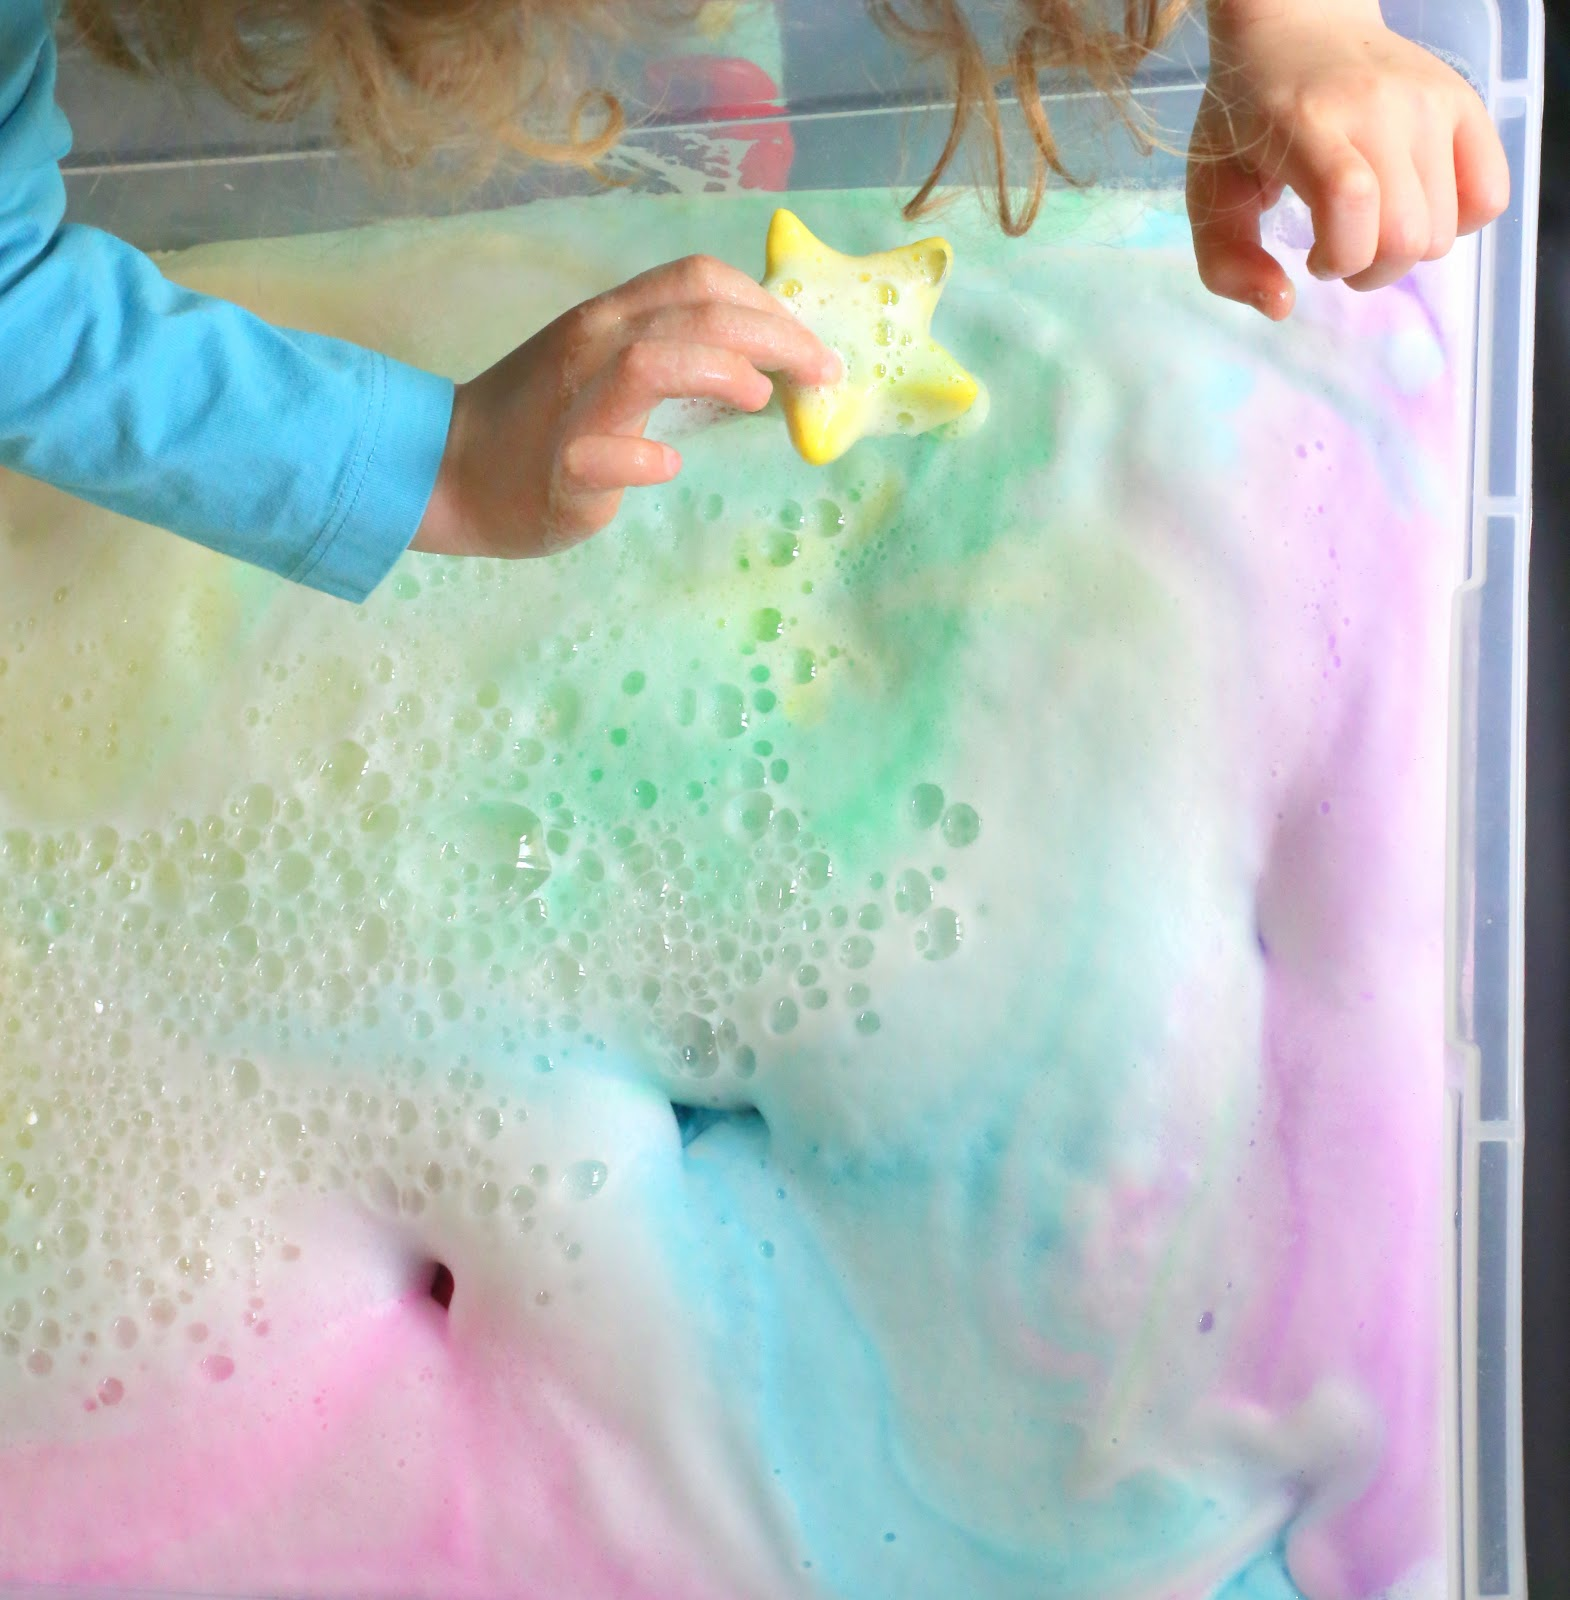
\includegraphics[scale=0.07]{1-IMG_4360.JPG}

{\tiny image © 2014 Asia Citro, reproduced with permission from \\
\url{http://www.funathomewithkids.com/2014/07/magic-foaming-treasure-stars.html}}
\end{figure}

\pause
\item \emph{siam twin matryoshkas}
\end{itemize}
\end{frame}
\begin{frame}{This work}
\begin{itemize}
  \item define and characterize notions of agreement --
  \emph{\textbf{refinement}, \textbf{local agreement} and \textbf{global
  agreement}}
  \item find the \textbf{computational complexity} of the
  \textbf{satisfiability} of the \emph{\textbf{monadic}} and the
  \emph{\textbf{two-variable}} fragment with respect to these notions
\end{itemize}
\end{frame}

\begin{frame}{Overview}
\tableofcontents
\end{frame}

\section{Setups}
\begin{frame}{Setups}
\begin{itemize}
  \item
   use unary predicate symbols to ``encode'' data at elements of structures
  
  \item
  example: a permutation setup ``encodes'' a permutation at every
  element of a structure
  
  \item
  $\text{bits} \to \text{binary counters} \to \text{vectors} \to
  \text{permutations}$
\end{itemize}
\end{frame}

\begin{frame}{Bit Setups}
The set of \emph{bits} is $\Bits = \set{0,1}$.
A \emph{bit setup} is a predicate signature $\BS = \seq{\su}$ consisting of a
single unary predicate symbol $\su$.
\begin{itemize}
  \item Given $\StrA$, define the function $\data\su\StrA :
  \domA\to\Bits$ by:
  \[
    \data\su\StrA a = \begin{cases}
      1 &\text{if } \StrA \vDash \su(a) \\
      0 &\text{otherwise.}
    \end{cases}
  \]
  
  \item
  If $\datad\in\Bits$, define the formula $\feqA\su\datad(\xx)$ by:
  \[
  \feqA\su\datad(\xx) = \begin{cases}
    \su(\xx) &\text{if } \datad = 1 \\
    \lnot\su(\xx) &\text{otherwise.}
  \end{cases}
  \]
  
  \item Property: $\StrA\vDash\feqA\su\datad(\ea)$ iff $\data\su\StrA\ea =
  \datad$.
\end{itemize}
\end{frame}

\begin{frame}{Bit Setups Formulas}
\begin{align*}
  \feq\su(\xx,\yy) &= \su(\xx) \lequ \su(\yy) \\
  \feqOI\su(\xx,\yy) &= \lnot \su(\xx) \land \su(\yy) \\
  \feqIO\su(\xx,\yy) &= \su(\xx) \land \lnot \su(\yy). \\
\end{align*}
\begin{itemize}
  \item
  $\StrA\vDash\feq\su(\ea,\eb)$ iff $\data\su\StrA\ea = \data\su\StrA\eb$.
  
  \item
  $\StrA\vDash\feqOI\su(\ea,\eb)$ iff $\data\su\StrA\ea = 0$ and
  $\data\su\StrA\eb = 1$.
  
  \item
  $\StrA\vDash\feqIO\su(\ea,\eb)$ iff $\data\su\StrA\ea = 1$ and
  $\data\su\StrA\eb = 0$.
\end{itemize}
\end{frame}

\begin{frame}{Counter Setups}
The set of \emph{$\tbit$-bit numbers} is $\Bitnumst = [0, 2^\tbit-1]$.
A \emph{$\tbit$-bit counter setup} is a predicate signature $\CS =
\seq{\suu1,\suu2,\dots,\suu\tbit}$ consisting of $\tbit$ unary predicate
symbols.
\begin{itemize}
  \item
  Given $\StrA$, define the function $\data\CS\StrA : \domA \to \Bitnumst$ that
  returns a $\tbit$-bit number for any $\ea\in\domA$ by:
  \[
    \data\CS\StrA\ea = \sum_{1 \leq \ii \leq \tbit} 2^{\ii-1} 
    \data{\suu\ii}\StrA\ea.
  \]
\end{itemize}
\end{frame}

\begin{frame}{Counter Setups Formulas}
We can define \emph{\textbf{small formulas}} with the following properties:
\begin{itemize}
  \item
  $\StrA\vDash\feqA\CS\datad(\ea)$ iff $\data\CS\StrA\ea = \datad$.
  
  \item
  $\StrA\vDash\feq\CS(\ea,\eb)$ iff $\data\CS\StrA\ea = \data\CS\StrA\eb$.
  
  \item
  $\StrA\vDash\fless\CS(\ea,\eb)$ iff $\data\CS\StrA\ea < \data\CS\StrA\eb$.
  
  \item
  $\StrA\vDash\fsucc\CS(\ea,\eb)$ iff $\data\CS\StrA\eb = 1 +
  \data\CS\StrA\ea$.
  
  \item
  $\StrA \vDash \fbetw\CS\datad\datae(\ea)$ iff
  $\datad \leq \data\CS\StrA\ea \leq \datae$.
\end{itemize}
\end{frame}

\begin{frame}{Vector Setups}
The set of \emph{$n$-dimensional $t$-bit vectors} is $\ntBitnums\nn\tbit$.
An \emph{$n$-dimensional $t$-bit vector setup} is a predicate signature  $\VS =
\seq{\suu{11}, \suu{12}, \dots, \suu{\nn\tbit}}$ of $(\nn\tbit)$ distinct unary
predicate symbols.
\begin{itemize}
  \item
  The \emph{counter setup $\VSp\posp$} of $\VS$ at position $\posp \in [1,\nn]$
  is $\VSp\posp = \seq{\suu{\posp1},\suu{\posp2},\dots,\suu{\posp\tbit}}$.
  
  \item
  $\data\VS\StrA\ea = \left(\data{\VSp1}\StrA\ea,\data{\VSp2}\StrA\ea, \dots,
  \data{\VSp\nn}\StrA\ea\right)$.
\end{itemize}
\end{frame}

\begin{frame}{Vector Setups \textbf{Small Formulas}}
\begin{itemize}
  \item
  $\StrA\vDash\feqP\VS\posp\posq(\ea)$ iff $\data{\VSp\posp}\StrA\ea =
  \data{\VSp\posq}\StrA\ea$.
  
  \item
  $\StrA\vDash\flessP\VS\posp\posq(\ea)$ iff $\data{\VSp\posp}\StrA\ea <
  \data{\VSp\posq}\StrA\ea$.
  
  \item
  $\StrA\vDash\fsuccP\VS\posp\posq(\ea)$ iff $\data{\VSp\posq}\StrA\ea =
  1 + \data{\VSp\posp}\StrA\ea$.
  
  \item
  antilexicographic ordering, e.g. $(1,1,0)\lexlt (0,0,1)$:
  $\StrA\vDash\fless\VS(\ea,\eb)$ iff
  $\data{\VS}\StrA\ea\lexlt\data{\VS}\StrA\eb$.
\end{itemize}
\end{frame}

\begin{frame}{Permutation Setups}
The set of permutations of $[1,n]$ is $\Perms\nn$.

Encode an $n$-permutation $\permnu\in\Perms\nn$ by the
$n$-dimensional $t$-bit vector $(\permnu(1), \permnu(2), \dots, \permnu(n))$,
where $t$ is the bitsize of $n$.

An \emph{$n$-permutation setup} $\PS =
\seq{\suu{11},\suu{12},\dots,\suu{nt}}$ is just an $n$-dimensional $t$-bit
vector.

The \emph{\textbf{small formula}} $\fperm\PS = \fbetw\PS1\nn \land \falldiff\PS$
asserts that the vector setup encodes exactly the permutations.
\end{frame}

\section{Equivalence Relations}
\begin{frame}{Agreement}
Let $\relEE1,\relEE2,\dots,\relEE\nn$ be a sequence of equivalence relations on
$\domA$. The sequence is in
\begin{itemize}
  \item
  \emph{refinement} if it forms a chain under
  inclusion,
  that is if $\relEE1\subseteq\relEE2\subseteq\dots\subseteq\relEE\nn$
  
  \pause
  \item
  \emph{global agreement} if it can be rearranged into
  a chain under inclusion,
  that is if $\relEE{\permnu(1)}\subseteq\relEE{\permnu(2)}\subseteq\dots
  \subseteq\relEE{\permnu(\nn)}$ for some permutation $\permnu$ of $[1,\nn]$
  
  \pause
  \item
  \emph{local agreement} if for every $\ea\in\domA$,
  the sequence of equivalence classes
  $\relEE1[\ea],\relEE2[\ea],\dots,\relEE\nn[\ea]$ can be rearranged into a
  chain under inclusion, that is if for every $\ea\in\domA$ there
  is some permutation $\permnu(\ea)$ of $[1,\nn]$ such that
  $\relEE{\permnu(\ea)(1)}[\ea]\subseteq\relEE{\permnu(\ea)(2)}[\ea]\subseteq
  \dots\subseteq\relEE{\permnu(\ea)(\nn)}[\ea]$
  
  \pause
  \item
  $\text{refinement} \implies \text{global agreement} \implies \text{local
  agreement}$
\end{itemize}
\end{frame}

\begin{frame}{Intuition}
Intuitively
\begin{itemize}
  \item 
  $\text{global agreement} = \text{refinement} + \text{a permutation}$
  
  \pause
  \item
  $\text{local agreement} = \text{refinement} + \text{locally agreeing
  permutations}$
\end{itemize}
\end{frame}

\begin{frame}{Example}
Example of a sequence $E_1, E_2, E_3$ in local agreement:

\begin{tikzpicture}
\fill[color=orange] (-1.5,-0.5) rectangle (1.5,2.5);
\draw (-1.5,-0.5) rectangle (1.5,2.5);
\node[below] at (-1.3,2.6) {$E_3$};
\fill[color=yellow] (-1,0) rectangle (1,2);
\draw (-1,0) rectangle (1,2);
\node[below] at (-0.8,2.1) {$E_2$};
\fill[color=green] (-0.5,0.5) rectangle (0.5,1.5);
\draw (-0.5,0.5) rectangle (0.5,1.5);
\node[below] at (-0.3,1.6) {$E_1$};

\fill (0,1) circle [radius=2pt];
\node[right] at (0,1) {$a$};

\fill[color=yellow] (2,-0.5) rectangle (7.5,2.5);
\draw (2,-0.5) rectangle (7.5,2.5);
\node[below] at (2.2,2.6) {$E_2$};

\fill[color=orange] (2.5,-0.2) rectangle (4.5,2.2);
\draw (2.5,-0.2) rectangle (4.5,2.2);
\node[below] at (2.7,2.3) {$E_3$};

\fill[color=green] (3,0) rectangle (4,0.9);
\draw (3,0) rectangle (4,0.9);
\node[below] at (3.2,1) {$E_1$};
\fill (3.5,0.45) circle [radius=2pt];
\node[right] at (3.5,0.45) {$b$};

\fill[color=green] (3,1.1) rectangle (4,2);
\draw (3,1.1) rectangle (4,2);
\node[below] at (3.2,2.1) {$E_1$};
\fill (3.5,1.55) circle [radius=2pt];

\fill[color=green] (5,-0.2) rectangle (7,2.2);
\draw (5,-0.2) rectangle (7,2.2);
\node[below] at (5.2,2.3) {$E_1$};

\fill[color=orange] (5.5,0) rectangle (6.5,0.9);
\draw (5.5,0) rectangle (6.5,0.9);
\node[below] at (5.7,1) {$E_3$};

\fill[color=orange] (5.5,1.1) rectangle (6.5,2);
\draw (5.5,1.1) rectangle (6.5,2);
\node[below] at (5.7,2.1) {$E_3$};
\fill (6,1.55) circle [radius=2pt];
\node[right] at (6,1.55) {$c$};

\draw (5.5,0) rectangle (6.5,0.9);
\fill[color=orange] (5.5,0) rectangle (6.5,0.9);
\node[below] at (5.7,1) {$E_3$};
\fill (6,0.45) circle [radius=2pt];
\end{tikzpicture}
\end{frame}

\begin{frame}{Characterization}
\begin{lemma}
The sequence $E_1, E_2$ of two equivalence relations on $A$ is in local
agreement iff $E_1\cup E_2$ is an equivalence relation on $A$.
\end{lemma}

\begin{theorem}
The sequence $E_1, E_2, \dots, E_n$ of equivalence relations on $A$ is in local
agreement iff the union of any nonempty subsequence is an equivalence relation
on $A$, that is for any $m \in [1,n]$ and $1 \leq i_1 < i_2 < \dots < i_m \leq
n$ we have that $E_{i_1} \cup E_{i_2} \cup \dots \cup E_{i_m}$ is an equivalence
relation on $A$.
\end{theorem}
\end{frame}

\begin{frame}{Levels}
The \emph{level sequence} $L_1,L_2,\dots,L_n$ of
the sequence $E_1,E_2,\dots,E_n$ of equivalence relations on $A$ in local
agreement is defined by:
\[
L_m = \bigcap\{E_{i_1} \cup E_{i_2} \cup \dots \cup E_{i_m} \mid 1\leq i_1 <
i_2 < \dots < i_m \leq n\}.
\]
\begin{remark}
The level sequence is a sequence of equivalence relations on $A$ in refinement.
\end{remark}
\end{frame}

\begin{frame}{Example}
\begin{tikzpicture}
\fill[color=orange] (-1.5,-0.5) rectangle (1.5,2.5);
\draw (-1.5,-0.5) rectangle (1.5,2.5);
\node[below] at (-1.3,2.6) {$E_3$};
\fill[color=yellow] (-1,0) rectangle (1,2);
\draw (-1,0) rectangle (1,2);
\node[below] at (-0.8,2.1) {$E_2$};
\fill[color=green] (-0.5,0.5) rectangle (0.5,1.5);
\draw (-0.5,0.5) rectangle (0.5,1.5);
\node[below] at (-0.3,1.6) {$E_1$};

\fill (0,1) circle [radius=2pt];
\node[right] at (0,1) {$a$};

\fill[color=yellow] (2,-0.5) rectangle (7.5,2.5);
\draw (2,-0.5) rectangle (7.5,2.5);
\node[below] at (2.2,2.6) {$E_2$};

\fill[color=orange] (2.5,-0.2) rectangle (4.5,2.2);
\draw (2.5,-0.2) rectangle (4.5,2.2);
\node[below] at (2.7,2.3) {$E_3$};

\fill[color=green] (3,0) rectangle (4,0.9);
\draw (3,0) rectangle (4,0.9);
\node[below] at (3.2,1) {$E_1$};
\fill (3.5,0.45) circle [radius=2pt];
\node[right] at (3.5,0.45) {$b$};

\fill[color=green] (3,1.1) rectangle (4,2);
\draw (3,1.1) rectangle (4,2);
\node[below] at (3.2,2.1) {$E_1$};
\fill (3.5,1.55) circle [radius=2pt];

\fill[color=green] (5,-0.2) rectangle (7,2.2);
\draw (5,-0.2) rectangle (7,2.2);
\node[below] at (5.2,2.3) {$E_1$};

\fill[color=orange] (5.5,0) rectangle (6.5,0.9);
\draw (5.5,0) rectangle (6.5,0.9);
\node[below] at (5.7,1) {$E_3$};

\fill[color=orange] (5.5,1.1) rectangle (6.5,2);
\draw (5.5,1.1) rectangle (6.5,2);
\node[below] at (5.7,2.1) {$E_3$};
\fill (6,1.55) circle [radius=2pt];
\node[right] at (6,1.55) {$c$};

\fill[color=orange] (5.5,0) rectangle (6.5,0.9);
\draw (5.5,0) rectangle (6.5,0.9);
\node[below] at (5.7,1) {$E_3$};
\fill (6,0.45) circle [radius=2pt];
\end{tikzpicture}

\begin{tikzpicture}
\fill[color=orange] (-1.5,-0.5) rectangle (1.5,2.5);
\draw (-1.5,-0.5) rectangle (1.5,2.5);
\node[below] at (-1.3,2.6) {$L_3$};
\fill[color=yellow] (-1,0) rectangle (1,2);
\draw (-1,0) rectangle (1,2);
\node[below] at (-0.8,2.1) {$L_2$};
\fill[color=green] (-0.5,0.5) rectangle (0.5,1.5);
\draw (-0.5,0.5) rectangle (0.5,1.5);
\node[below] at (-0.3,1.6) {$L_1$};

\fill (0,1) circle [radius=2pt];
\node[right] at (0,1) {$a$};

\fill[color=orange] (2,-0.5) rectangle (7.5,2.5);
\draw (2,-0.5) rectangle (7.5,2.5);
\node[below] at (2.2,2.6) {$L_3$};

\fill[color=yellow] (2.5,-0.2) rectangle (4.5,2.2);
\draw (2.5,-0.2) rectangle (4.5,2.2);
\node[below] at (2.7,2.3) {$L_2$};

\fill[color=green] (3,0) rectangle (4,0.9);
\draw (3,0) rectangle (4,0.9);
\node[below] at (3.2,1) {$L_1$};
\fill (3.5,0.45) circle [radius=2pt];
\node[right] at (3.5,0.45) {$b$};

\fill[color=green] (3,1.1) rectangle (4,2);
\draw (3,1.1) rectangle (4,2);
\node[below] at (3.2,2.1) {$L_1$};
\fill (3.5,1.55) circle [radius=2pt];

\fill[color=yellow] (5,-0.2) rectangle (7,2.2);
\draw (5,-0.2) rectangle (7,2.2);
\node[below] at (5.2,2.3) {$L_2$};

\fill[color=green] (5.5,0) rectangle (6.5,0.9);
\draw (5.5,0) rectangle (6.5,0.9);
\node[below] at (5.7,1) {$L_1$};

\fill[color=green] (5.5,1.1) rectangle (6.5,2);
\draw (5.5,1.1) rectangle (6.5,2);
\node[below] at (5.7,2.1) {$L_1$};
\fill (6,1.55) circle [radius=2pt];
\node[right] at (6,1.55) {$c$};

\fill[color=green] (5.5,0) rectangle (6.5,0.9);
\draw (5.5,0) rectangle (6.5,0.9);
\node[below] at (5.7,1) {$L_1$};
\fill (6,0.45) circle [radius=2pt];
\end{tikzpicture}
\end{frame}

\begin{frame}{Permutations}
\begin{lemma}
Let $E_1,E_2,\dots,E_n$ be a sequence of equivalence relations on $A$ in local
agreement having level sequence $L_1,L_2,\dots,L_n$.
Suppose that $a \in A$ and that $\nu$ is any permutation witnessing the local
agreement at $a$:
\[
E_{\nu(1)}[a] \subseteq E_{\nu(2)}[a] \subseteq \dots \subseteq E_{\nu(n)}[a].
\]
Then $L_k[a] = E_{\nu(k)}[a]$ for any $k\in[1,n]$.
\end{lemma}
\end{frame}

\section{Reductions}
\begin{frame}{Notation}
\[
  \Lvp\LL\nv\pow\Eea\sze\ag
\]
\begin{itemize}
  \item
  $\LL$, the \emph{ground logic}, is the first-order logic with formal equality
  
  \pause
  \item
  $\nv$, if given, bounds the number of allowed variables
  
  \pause
  \item
  $\sze$, if given, specifies the number of builtin equivalence symbols
  
  \pause
  \item
  $\ag\in\set{\agrefine,\agglobal,\aglocal}$, if given, specifies the agreement
  condition between the equivalence symbols
  
  \pause
  \item
  if $\pow$ is not given, the signature consists of arbitrary many unary and
  binary predicate symbols
  
  \pause
  \item
  if $\pow = 0$, the signature consists of only constantly many unary predicate
  symbols
  
  \pause
  \item
  if $\pow = 1$, the signature consists of arbitrary many unary predicate
  symbols
\end{itemize}
\end{frame}

\begin{frame}{Examples}
\begin{itemize}
  \item
  $\Lvp\LL\nonv0\Eea1\noag$ is the logic of a single equivalence
  
  \item
  $\Lvp\LL\nonv1$ is the monadic fragment
  
  \item
  $\Lvp\LL2\nopow\Eea2\aglocal$ is the two-variable logic featuring unary and
  binary predicate symbols in addition to two builtin equivalence symbols in
  local agreement
\end{itemize}
\end{frame}

\begin{frame}{Reduction Strategy}
To reduce $\FinASat{\Lvp\LL\nonv\nopow\Eea\sze\aglocal}$ to
$\FinASat{\Lvp\LL\nonv\nopow\Eea\sze\agrefine}$,
\begin{itemize}
  \item
  look at the levels
  
  \item
  encode a permutation witnessing the local agreement in a permutation setup
  
  \item
  define formulas that recover the original equivalences from the
  levels and the permutations
  
  \item
  not every combination of levels and permutations defines
  local agreement $\implies$ need constraint on permutations
\end{itemize}
\end{frame}

\begin{frame}{Characteristic Permutations}
Consider an $\Lvp\LL\nonv\nopow\Eea\sze\aglocal$-signature $\Sigma$ containing
$\ES = \seq{\see1,\see2,\dots,\see\sze}$.
Let $\StrA$ be a $\Sigma$-structure, $\relEE\ii =
\at\StrA{\see\ii}$ and $\ea\in\domA$.

The \emph{characteristic permutation} $\nu$ at $\ea$ is the
antilexicographically smallest permutation of $[1,e]$ satisfying:
\[
\relEE{\nu(1)}[a] \subseteq \relEE{\nu(2)}[a] \subseteq \dots
\subseteq \relEE{\nu(\sze)}[a].
\]
Collect the characteristic permutations in $\chperm\Sigma\StrA : \domA \to
\Perms\sze$.
\end{frame}

\begin{frame}{Local Agreement of Permutations}
\begin{remark}
Let $\relLL1,\relLL2,\dots,\relLL\sze$ be the levels of $\relEE\ii$,
$\ea,\eb\in\domA$,
$\perma = \chperm\Sigma\StrA\ea$
and $\permb = \chperm\Sigma\StrA\eb$.

If $(\ea,\eb)\in\relLL\kk$, then $\perma(\kk) = \permb(\kk)$.

That is, if $\ea$ and $\eb$ are connected at level $\kk$, then their
characteristic permutations agree at position $\kk$.
\end{remark}
\begin{itemize}
  \item
  This doesn't hold in general for any set of witnessing permutations
\end{itemize}
\end{frame}

\begin{frame}{Levels and Permutations}
Let $\LS = \seq{\slee1,\slee2,\dots,\slee\sze} + \PS$ consist of the builtin
equivalence symbols $\slee\ii$ (we intend to interpret them as the levels)
together with the permutation setup $\PS$ (intended to encode the
characteristic permutations).

The formula
\[
  \ffixperm\LS = \forall\xx \forall\yy \bigwedge_{1 \leq \kk \leq \sze}
  \left(\slee\kk(\xx,\yy) \limp \feq{\PSp{\kk}}(\xx,\yy)\right).
\]
encodes the local agreement of permutations.
\end{frame}

\begin{frame}{Recovering}
The formulas
\[
  \fel\LS\ii(\xx,\yy) = \bigwedge_{1 \leq \kk \leq \sze}
  \left(\feqA{\PS(\kk)}\ii(\xx) \limp \slee\kk(\xx,\yy)\right)
\]
recover the original equivalences ($\ii\in[1,\sze]$).
\begin{remark}
Let $\StrA$ be an $\LS$-structure satisfying
$\fperm\PS\land\ffixperm\LS$ such that the level symbols $\slee\ii$ are
interpreted as a sequence of equivalence relations in refinement.
Let $\relLL\ii = \at\StrA{\slee\ii}$ and $\relEE\ii = \at\StrA{\fel\LS\ii}$.

Then $\relEE\ii$ is a sequence of equivalence relations in local agreement and
$\relLL\kk[\ea] = \relEE{\perma(\kk)}[\ea]$ for any $\ea\in\domA$ and $\perma =
\data\PS\StrA$.
\end{remark}
\end{frame}

\begin{frame}{Translation}
Let $\Sigma' = \Sigma + \LS$ and $\LS' = \Sigma' - \ES$.
The translation $\ltr\fphi : \FoF\Sigma \to \FoF\LSp$ is defined by
\[
  \ltr\fphi = \fphip \land \fperm\PS \land \ffixperm\LS,
\]
where $\fphip$ is obtained from $\fphi$ by replacing all occurrences
of $\see\ii(x,y)$ by $\fel\LS\ii(x,y)$.
\begin{remark}
$\fphi$ is (finitely) satisfiable over $\Lvp\LL\nonv\nopow\Eea\sze\aglocal$ iff
$\ltr\fphi$ is (finitely) satisfiable over
$\Lvp\LL\nonv\nopow\Eea\sze\agrefine$.
\end{remark}
\begin{itemize}
  \item
  if $\StrA\vDash\fphi$, interpret $\slee\ii$ as the levels and encode
  $\chperm\Sigma\StrA$ in the permutation setup $\PS$.
  
  \item
  if $\StrAp\vDash\ltr\fphi$, interpret $\see\ii$ as $\fel\LS\ii$.
\end{itemize}
\end{frame}

\begin{frame}{Translation}
The translation just uses polynomially many new unary predicate symbols (it can
``reuse'' the builtin equivalences).
\begin{proposition}
\begin{itemize}
  \item
  the logic $\Fo\Eea\sze\aglocal$ has the finite model property iff
  the logic $\Fo\Eea\sze\agrefine$ has the finite model property
  
  \item
  the corresponding satisfiability problems are polynomial-time equivalent
  
  \item
  also works for $\Lvp\LL\nonv1\Eea\sze\aglocal$ and
  $\Lvp\LL2\nopow\Eea\sze\aglocal$
\end{itemize}
\end{proposition}
\end{frame}

\section{Monadic Logics}
\begin{frame}

{\LARGE Monadic Logics}
\end{frame}
\begin{frame}{Results}
It is known that:
\begin{itemize}
  \item
  $\Lvp\LL\nonv1$ has the finite model property~{[L{\"o}wenheim 1915]} and
  its satisfiability problem is $\cNExpTime$-complete
  
  \pause
  \item
  $\Lvp\LL\nonv0\Eea1\noag$ has the finite model property and
  its satisfiability problem is $\cPSpace$-complete
  
  \pause
  \item
  $\Lvp\LL\nonv0\Eea2\noag$ lacks the finite model property
  and both the satisfiability and finite satisfiability are
  undecidable~{[Janiczak 1953]}
\end{itemize}

\pause
How about $\Lvp\LL\nonv1\Eea1\noag$?
\pause
\textbf{We show that:}
\begin{itemize}
  \item\textbf{
  $\Lvp\LL\nonv1\Eea1\noag$ has the finite model property and its
  satisfiability problem is $\ceNExpTime2$-complete}
  
  \item\textbf{
  in general, $\Lvp\LL\nonv1\Eea\sze\agrefine$ has the finite model property and
  its satisfiability problem is $\ceNExpTime{(\sze+1)}$-complete}
\end{itemize}
\end{frame}

\begin{frame}{Complexity: Cells}
\begin{columns}[T]
\begin{column}{0.42\textwidth}
Let $\Sigma = \seq{\suu1,\suu2,\dots,\suu\szu,\se}$ and $\StrA$ be a
$\Sigma$-structure.

A \emph{cell} $C\subseteq\domA$ is a maximal set of $\se$-equivalent elements
satisfying the same $\su$-predicates.
\end{column}%
\begin{column}{0.6\textwidth}
Example $\Sigma = \seq{\suu1,\suu2,\se}$

\begin{tikzpicture}
\draw[style=thick] (0,-2) rectangle (4,2);
\node[above right] at (0,2) {$E[a]$};

\draw[style=dashed] (0,0) rectangle (2,2);
\node[below right] at (0,2) {$\suu1,\suu2$};
\draw[fill] (0.5,0.5) circle [radius=2pt];
\draw[fill] (1.5,0.5) circle [radius=2pt];
\draw[fill] (0.5,1.5) circle [radius=2pt];
\draw[fill] (1.5,1.5) circle [radius=2pt];
\node[right] at (0.5,0.5) {$a$};

\draw[style=dashed] (2,0) rectangle (4,2);
\node[below right] at (2,2) {$\lnot\suu1,\suu2$};
\draw[fill] (2.5,1) circle [radius=2pt];
\draw[fill] (3.5,1) circle [radius=2pt];

\node[below right] at (0,0) {$\lnot\suu1,\lnot\suu2$};
\draw[fill] (2,-1) circle [radius=2pt];

\draw[style=thick] (4,-2) rectangle (6,2);
\node[above right] at (4,2) {$E[b]$};
\node[below right] at (4,2) {$\lnot\suu1,\lnot\suu2$};
\draw[fill] (5,1) circle [radius=2pt];
\node[right] at (5,1) {$b$};
\draw[fill] (5,0) circle [radius=2pt];
\draw[fill] (5,-1) circle [radius=2pt];
\end{tikzpicture}
\end{column}%
\end{columns}
\end{frame}

\begin{frame}{Small Cells}
\begin{lemma}
Let $\nr \geq 1$ and suppose that $\StrA$ is a $\Sigma$-structure.
Then there is a substructure $\StrB\subseteq\StrA$ such that
$\StrB\requiv\nr\StrA$ and every $\StrB$-cell has cardinality at most $\nr$.
\end{lemma}
\begin{proof}[Proof Idea]
For every $\StrA$-cell, if it has less than $\nr$ elements select them all,
otherwise select any $\nr$ elements. Consider $\StrB$ induced by the selected
elements.
Win the \emph{$\nr$-round Ehrenfeucht-Fra\"{i}ss\'{e} game} as Duplicator:
if the challenge is new, choose a new selected element from the same cell.
Since the game lasts $\nr$ rounds, you'll never run out of selected elements.
\end{proof}
\end{frame}

\begin{frame}{Few Isomorphic Classes}
\begin{lemma}
Let $\nr \geq 1$ and suppose that $\StrA$ is a $\Sigma$-structure.
Then there is a substructure $\StrB\subseteq\StrA$ such that
$\StrB\requiv\nr\StrA$ and $\StrB$-class is isomorphic to at most $(\nr-1)$
other $\StrB$-classes.
\end{lemma}

Combining these and doing the math, we get:
\begin{remark}
Let $\StrA$ be a $\Sigma(\szu,1)$-structure and let $\nr\geq1$.
There is some $\StrB\subseteq\StrA$ such that $\StrB\requiv\nr\StrA$ and
$\card\domB \leq r^2 2^u ((r+1)^{2^u}-1)$.
\end{remark}

This is doubly exponential with respect to the size of $\fphi$, hence
$\FinASat{\Lvp\LL\nonv1\Eea1\noag}$ is in $\ceNExpTime2$.
\end{frame}

\begin{frame}{Hardness: Domino Problem}
\begin{itemize}
  \item 
Reduce the $\ceNExpTime2$-complete Square Domino Tiling Problem to
$\FinASat{\Lvp\LL\nonv1\Eea1\noag}$.

\item
A \emph{domino system} is a triple $D = (T,H,V)$, where
$T = [1,k]$ is a set of \emph{tiles} and $H,V\subseteq T\cprod T$ are the
\emph{horizontal} and \emph{vertical matching relations}.

\item
A \emph{tiling} of the $m\cprod m$ square for a domino system $D$ with initial
condition $c^0 = \seq{t_1^0,t_2^0,\dots,t_n^0}$, where $n\leq m$, is a mapping
$t : [1,m]\cprod [1,m]\to T$ such that:
\begin{itemize}
  \item $(t(i,j),t(i+1,j))\in H$ for all $i\in[1,m-1], j\in[1,m]$
  \item $(t(i,j),t(i,j+1))\in V$ for all $i\in[1,m], j\in[1,m-1]$
  \item $t(i,1) = t_i^0$ for all $i\in[1,n]$
\end{itemize}
\end{itemize}
\end{frame}

\begin{frame}{Domino Problem}
Example $T = [1,3]$, $H = \set{(1,3),(2,1),(2,2)}, V = \set{(2,2),(3,2),(1,2)}$

\centering
\begin{tikzpicture}
\draw[->] (-0.2,0.2) to (-0.2,1.8);
\draw[->] (0.2,-0.2) to (1.8,-0.2);
\draw (0,0) rectangle (1,1);
\draw (1,0) rectangle (2,1);
\draw (0,1) rectangle (1,2);
\draw (1,1) rectangle (2,2);
\node at (0.5,0.5) {$1$};
\node at (1.5,0.5) {$3$};
\node at (0.5,1.5) {$2$};
\node at (1.5,1.5) {$2$};

\end{tikzpicture}

\begin{theorem}
There is a domino system $D_0$ such that the problem of asking if there exists a
tiling for $D_0$ with initial condition $c_0$ of length $n$ for the
$2^{2^n}\cprod 2^{2^n}$-square is $\ceNExpTime2$-complete.
\end{theorem}
\end{frame}

\begin{frame}{Hardness}
Main issue: given $\Sigma = \seq{\suu1,\suu2,\dots,\suu\szu,\se}$,
how can we define a doubly exponential grid?
\pause
\begin{itemize}
  \item
  Each class can contain exponentially many cells
  
  \item
  If we encode bits in cells, the classes encode doubly exponential numbers
\end{itemize}
\end{frame}

\begin{frame}{Encoding}
\begin{itemize}
  \item
  we can ensure that every class contains maximally many $2^u$ cells
  
  \item
  a cell containing a single element encodes bit $0$:
  \[
    \fbitO\Sigma(\xx) = \forall\yy \left(
    \se(\yy,\xx) \land \fposeq\Sigma(\yy,\xx) \limp \yy = \xx\right)
  \] 
  
  \item
  a cell containing more elements encodes bit $1$:
  \[
    \fbitI\Sigma(\xx) = \exists\yy \left(
    \se(\yy,\xx) \land \fposeq\Sigma(\yy,\xx) \land \yy \neq \xx\right)
  \]
\end{itemize}
\end{frame}

\begin{frame}{Data}
Let $\StrA$ be a $\Sigma$-structure and let $\relE = \at\StrA\se$.
The equivalence classes of $\relE$ are $\Ecl\relE$.
The number encoded by the bitstring $\bstrb$ is $\bdec{\bstrb}$.

With \emph{a bit of work} we can define:
\begin{itemize}
  \item
  $\Data\Sigma\StrA : \Ecl\relE \to \tBitstrings{2^\szu}$ that assigns
  exponential bitstrings (hence doubly exponential numbers) to the classes of
  $\StrA$
  
  \item $\StrA\vDash\fZero\Sigma(\ea)$ iff
  $\bdec{\Data\Sigma\StrA{\relE[\ea]}} = 0$
  
  \item $\StrA\vDash\fSucc\Sigma(\ea,\eb)$ iff
  $\bdec{\Data\Sigma\StrA{\relE[\eb]}} = 1 +
  \bdec{\Data\Sigma\StrA{\relE[\ea]}}$
  
  \item etc.
\end{itemize}
\end{frame}

\begin{frame}{Reduction}
Given $D_0 = (T,V,H)$, where $T = [1,k]$, and $c^0 =
\seq{t_1^0,t_1^0,\dots,t_n^0}$, consider:
\begin{align*}
\Sigma &=
\seq{\suu1^H,\suu2^H,\dots,\suu\nn^H;\suu1^V,\suu2^V,\dots,\suu\nn^V;
\suu1^T,\suu2^T,\dots,\suu{k}^T;\se} \\
 &\suu1^T,\suu2^T,\dots,\suu{k}^T \text{for tiles} \\
\Sigma^{HV} &=
\seq{\suu1^H,\suu2^H,\dots,\suu\nn^H;\suu1^V,\suu2^V,\dots,\suu\nn^V;\se}
\text{for the full grid}
 \\
\Sigma^{H} &=
\seq{\suu1^H,\suu2^H,\dots,\suu\nn^H;\se} \text{for horizontal matching} \\
\Sigma^{V} &=
\seq{\suu1^V,\suu2^V,\dots,\suu\nn^V;\se} \text{for vertical matching}
\end{align*}
\end{frame}

\begin{frame}{Reduction}
\textbf{small formulas}
\begin{itemize}
  \item
  $\fposfull{\Sigma^{HV}}\land\fFull{\Sigma^{HV}}\land\fAlldiff{\Sigma^{HV}}$
  defines a full doubly exponential grid
  \item $
      \forall\xx \left(\bigvee_{1 \leq \ii \leq \kk} \left(\suuu\tiles\ii(\xx)
  \land \bigwedge_{\jj\in[1,\kk]\sub\set\ii}
  \lnot\suuu\tiles\jj(\xx)\right)\right)$ asserts that every element has a
  unique type
  \item $\forall\xx\forall\yy \Big(\se(\xx,\yy) \limp
  \bigwedge_{1 \leq \ii \leq \kk} 
  (\suuu\tiles\ii(\xx) \lequ \suuu\tiles\ii(\xx))\Big)$ asserts that the type is
  the same in each class
\end{itemize}
\end{frame}

\begin{frame}{Reduction}
\textbf{small formulas}
\begin{itemize}
  \item $\forall\xx \Big(\fDataA{\DS^\horm}{(\jj-1)}(\xx) \land \fZero{\DS^\verm}(\xx)
  \limp \suuu\tiles{\icondt\jj}(\xx)\Big)$ encodes the inital condition
  \item $\forall\xx\forall\yy \Big(\fSucc{\DS^\horm}(\xx,\yy) \land
  \fEq{\DS^\verm}(\xx,\yy) \limp
  \bigvee_{(\ii,\jj) \in \horm} \suuu\tiles{\ii}(\xx) \land
  \suuu\tiles{\jj}(\yy)\Big)$ encodes the horizontal tiling condition
\end{itemize}
\end{frame}

\begin{frame}{Summary}
\begin{itemize}
  \item
  this shows that the satisfiability of $\vFo2\Eea1\noag$ is $\ceNExpTime2$-hard
  
  \item
  the argument can be generalized and applied by induction to show that 
  the satisfiability of $\vFo2\Eea\sze\agrefine$ is $\ceNExpTime{(\sze+1)}$-hard
\end{itemize}
\end{frame}
\end{document}